\paragraph{Tuning Parameters}
\todo{Corrado: Did not see any algorithm so far. It’s hard to map these parameters to something I did not see yet jk}
The algorithm has four tuning parameters that can be tweaked; first, the \textit{step size}, the maximal normalized distance between connected samples in the connectivity trees, see \Cref{subfig:mp_step_size} \todo{Corrado: Put more of simple images as you go instead of a gigantic one later on }for a visual example. Choosing a high step size will increase search speed because the connectivity trees grow faster. A higher step size comes at the cost of smoothness; the resulting path will be bumpier with sharper corners.\todo{Corrado: Additionally, .. not Not a sentence } Additionally, the path has an increased chance of collision with obstacles because, for two connected configurations in a path, the individual configurations can both lie in free space. The space between configurations is not checked, and an obstacle could be in between the configurations, especially when cutting corners around obstacles. The second tuning parameter is the \textit{search size}, which is a subspace around the newly sampled sample (see, \Cref{subfig:mp_search_size}). In this subspace, a parent node is sought, and rewiring occurs. A parent node connects a new node with an edge to a connectivity tree. After connecting the new node to its parent node, rewiring occurs, changing the parent node by removing and adding an edge. If that results in a lower cost for that node, rewiring can be visually seen in \Cref{subfig:mp_rewire}. Increasing the search size improves the choice of the parent node and improves cost due to rewiring, but it also exponentially increases computation time. The third and fourth tuning parameters are the fixed costs for crossing through movable or unknown space, \Cref{fig:mp_push_or_drive} clearly shows the effect of varying such costs.\bs

The Pseudocode of the proposed algorithm is provided in \Cref{pseudocode:proposed_rrt_star}. The variables and /Rfunctions used are elaborated upon in the following \Cref{table:functions_for_proposed_rrt_star}.\bs


\todo{Corrado: I understand your attempt but reading the thesis as a whole asking to match colors with a picture is a lot to ask to a reader. I suggest the following: 

Before starting explaining just add an overall algorithm which is basically algorithm 1 where you have 1 sub-algorithm name per color. 

Then, when you explain the figure and the tuning parameters, as you go in the text you add pictures and sub algorithm. So a reader can incrementally add details to an already explained structure 
/}


\begin{figure}[H]
    \centering
    \begin{subfigure}{0.5\textwidth}
    \centering
    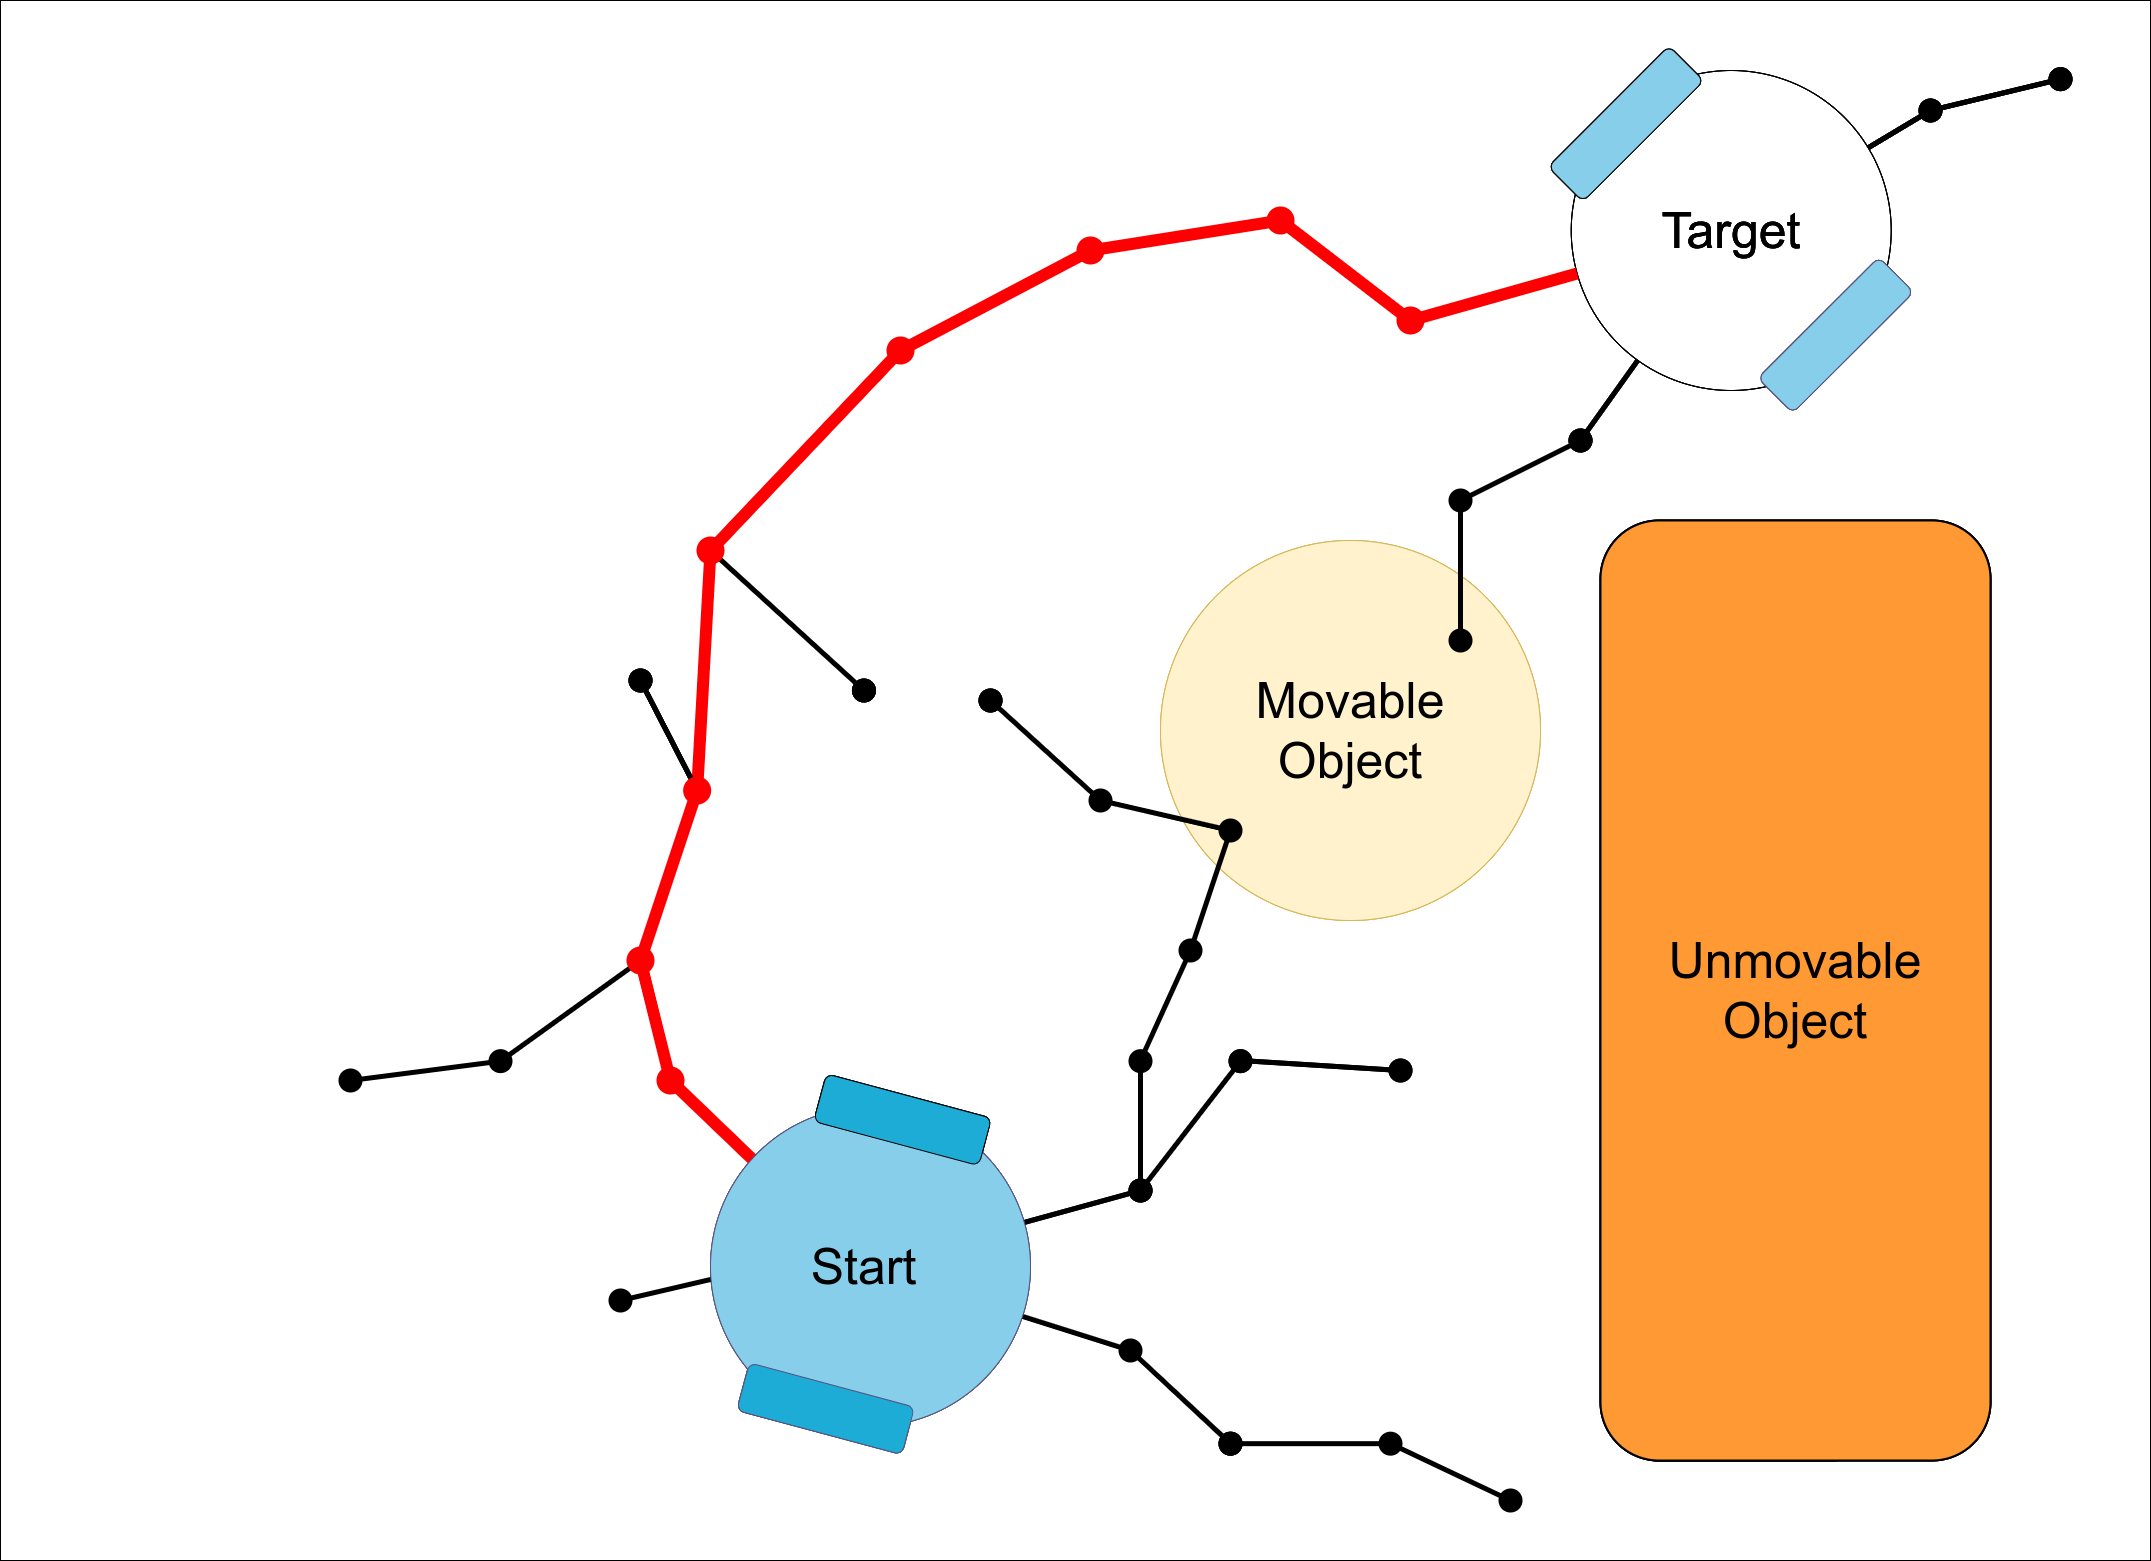
\includegraphics[width=1.10\textwidth]{figures/required_background/mp/7mp_path_found.drawio.png}
    \caption{Motion planner found a path found marked in red.}
    \end{subfigure}%

    \begin{subfigure}{\textwidth}
    \hspace{-0.7cm}
    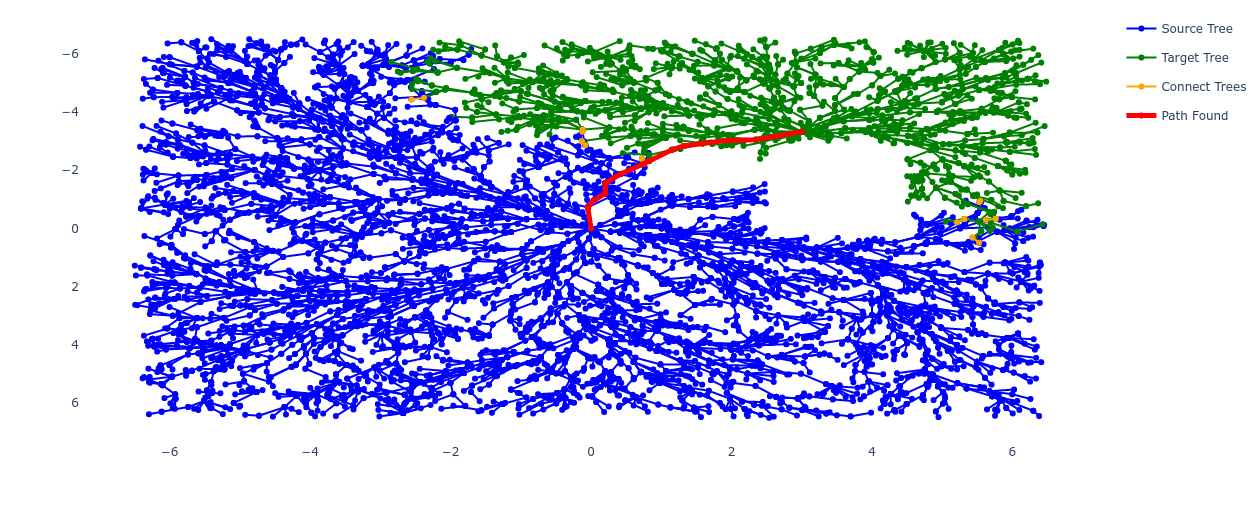
\includegraphics[width=1.1\textwidth]{figures/required_background/mp/mp_the_real_deal.png}
    \caption{A visualization of the implemented \acs{RRT*} algorithm\\when the stopping criteria was reached.}
    \end{subfigure}
    \label{fig:motion_planner_comparison}%
    \caption{Comparing schematic example to a visualization of the real algorithm.}
\end{figure}
\todo{Corrado: The caption here above is vague}

The added fixed cost for a path crossing through a movable or unknown object motivates the motion planner to find the shortest path around objects but prefers moving an object over making a large detour. Tuning the additional fixed cost for a path crossing through movable or unknown space balances the robot's decision between how long of a detour the robot is willing to drive, compared to pushing an object to free the path. Removing an unknown object bears more uncertainty than a movable object, which is why the additional cost to remove an unknown object is higher than that of a movable object. 
\todo{Corrado: So what’s your approach? Is there a systematic way or approach you used to tune this?}

\begin{figure}[H]

    \centering
    \begin{subfigure}{\textwidth}
    \centering
    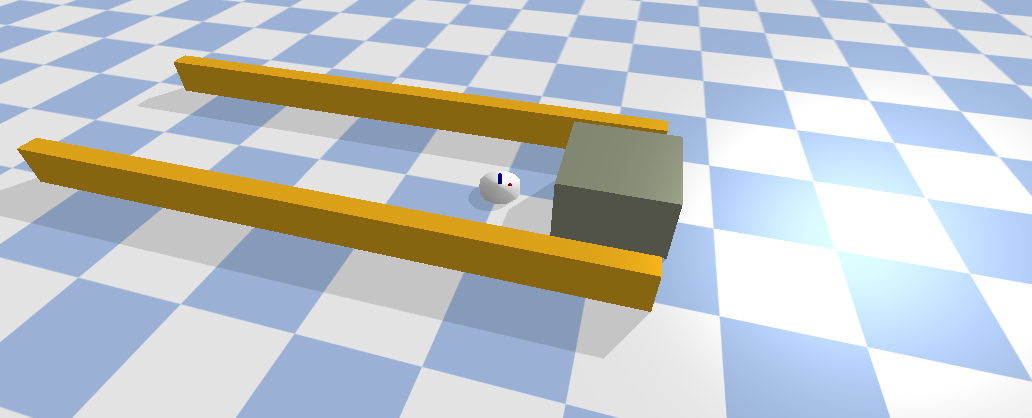
\includegraphics[width=0.9\textwidth]{figures/required_background/push_or_drive} \caption{Robot environment with the point robot, two yellow unmovable walls and an unknown brown box.}
    \end{subfigure}

    \begin{subfigure}{1.11\textwidth}
    \centering
    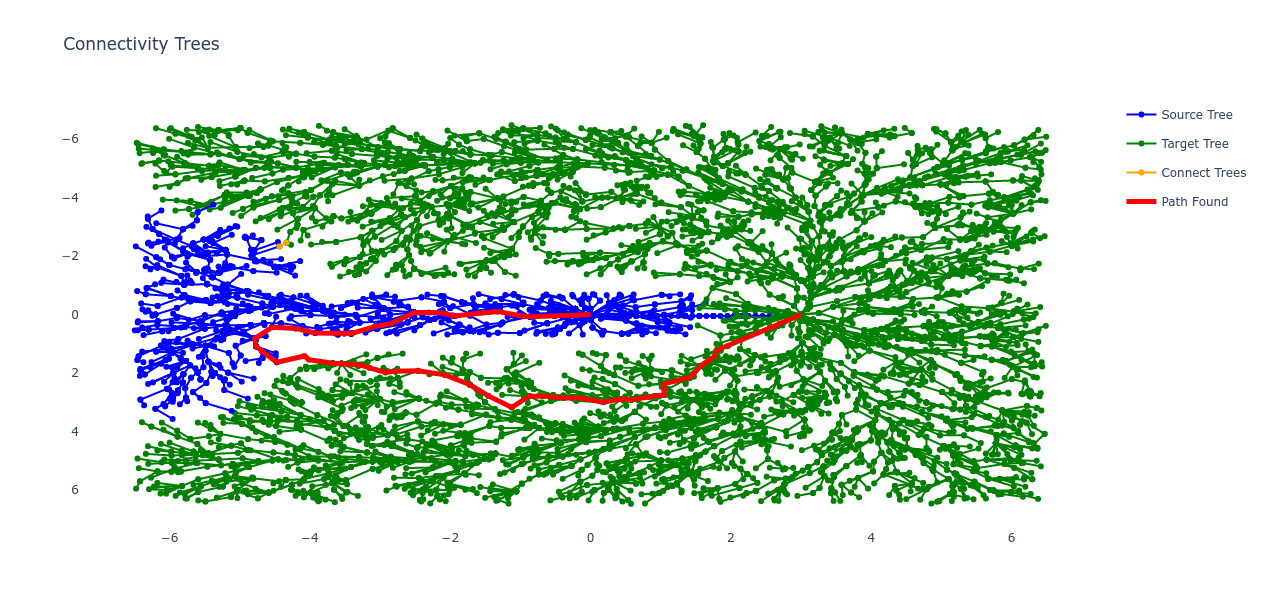
\includegraphics[width=\textwidth]{figures/required_background/mp/mp_high_fixed_cost}
    \caption{planned path around the brown box and yellow obstacles, with $\textrm{unknownSpaceCost} = 2$.}
    \end{subfigure}

    \begin{subfigure}{1.11\textwidth}
    \centering
    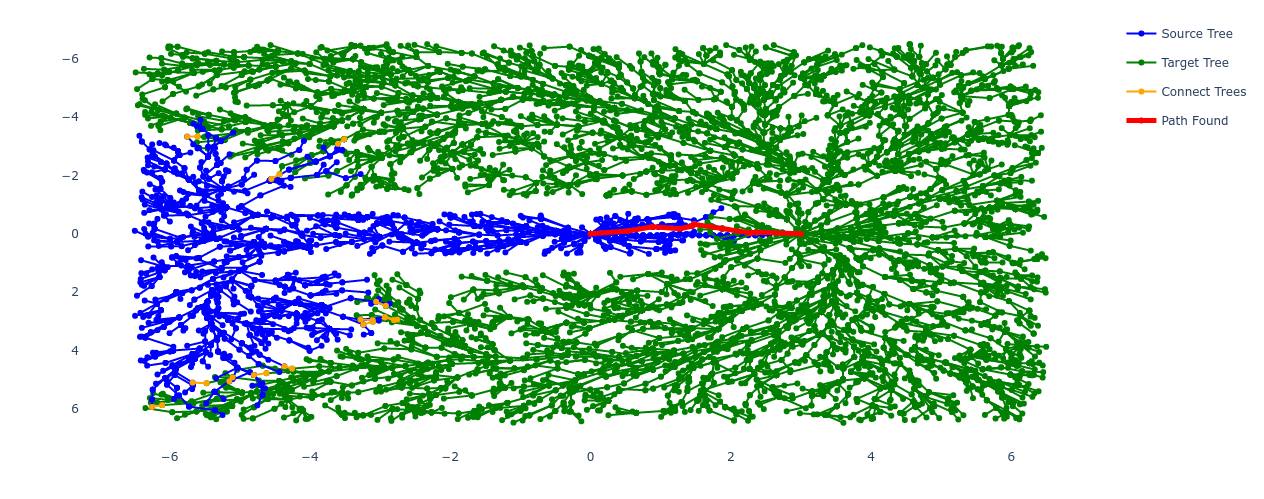
\includegraphics[width=\textwidth]{figures/required_background/mp/mp_low_fixed_cost}
    \caption{planned path going through the brown box, $\textrm{unknownSpaceCost} = 0.5$.}
    \end{subfigure}
    \caption{The robot tasked with driving toward the other side of the brown box.}%
    \label{fig:mp_push_or_drive}
\end{figure}

\todo{Corrado: a top view would be nice of that above thingy... easy to map to the ones just below}

The \todo{Corrado: It’s not a property of your proposed method per se but rather one of double rat star right?} proposed motion planning algorithm searches the configuration space from the start to target connectivity trees. Exploring faster than the single tree \ac{RRT*} algorithm \todo{Corrado: Do you have a reference for this? } because two trees grow and explore faster than a single tree. The proposed algorithm rewires nodes, lowering the cost for existing paths and convert to the optimal lowest-cost path with infinite sampling. System constraints are ensured by the \textit{ReachabilityCheck}\todo{Corrado: ReachabilityCheck, is nto explained at all} that validates if a node is reachable from another node using system models.\bs


The proposed algorithm yields feasible paths (according to the system model used to check reachability) that respect the system constraints. The algorithm prevents planning a path through blocking objects except when no other option is available or a large detour can be prevented. There are no performance tests taken on the modified motion planner other than visual inspection.
\todo{Corrado: So why should we believe the things you said so far about your proposed algorithm?}
For performance tests and comparison with equivalent sample-based state-of-the-art motion planners, see~\cite{chen_fast_2018}. Now that motion planning is discussed for drive actions, manipulation will be discussed for push actions.



\subsection{Manipulation Planning}%
\label{subsec:manipulation_planning}
With a push, two objects are primarily involved, the pushed object and the robot. Generally, and in this thesis, the pushed object's configuration is more important than the robot's configuration. The robot is only a means to push the object toward the target configuration. At which final configuration the robot itself ends up is of lesser importance. As long as during the push, the robot does not collide with objects other than the pushed object, and constraints on the robot must be respected.\bs

To plan a path that respects the constraints, \todo{Corrado: What does this mean? ->} the robot's configuration is generated for every newly added sample in the manipulation planning algorithm. 

\todo{Gijs For reachbailbpcheck, These lines just point out the name of the function again , there is no added information }
The \textit{ReachabilityCheck()} (see \Cref{table:functions_for_proposed_rrt_star} and line 33 in \Cref{pseudocode:proposed_rrt_star}) generates the robot configuration to validate if a new sample is reachable from an existing sample. This additional configuration is stored to create only feasible paths that respect the applied constraints. When the stopping criteria are reached and the shortest path is found, the generated robot configurations are discarded. \Cref{fig:manipulation_plannig_local_planner} displays a visual example of the procedure.\bs

\begin{figure}[H]
    \centering
    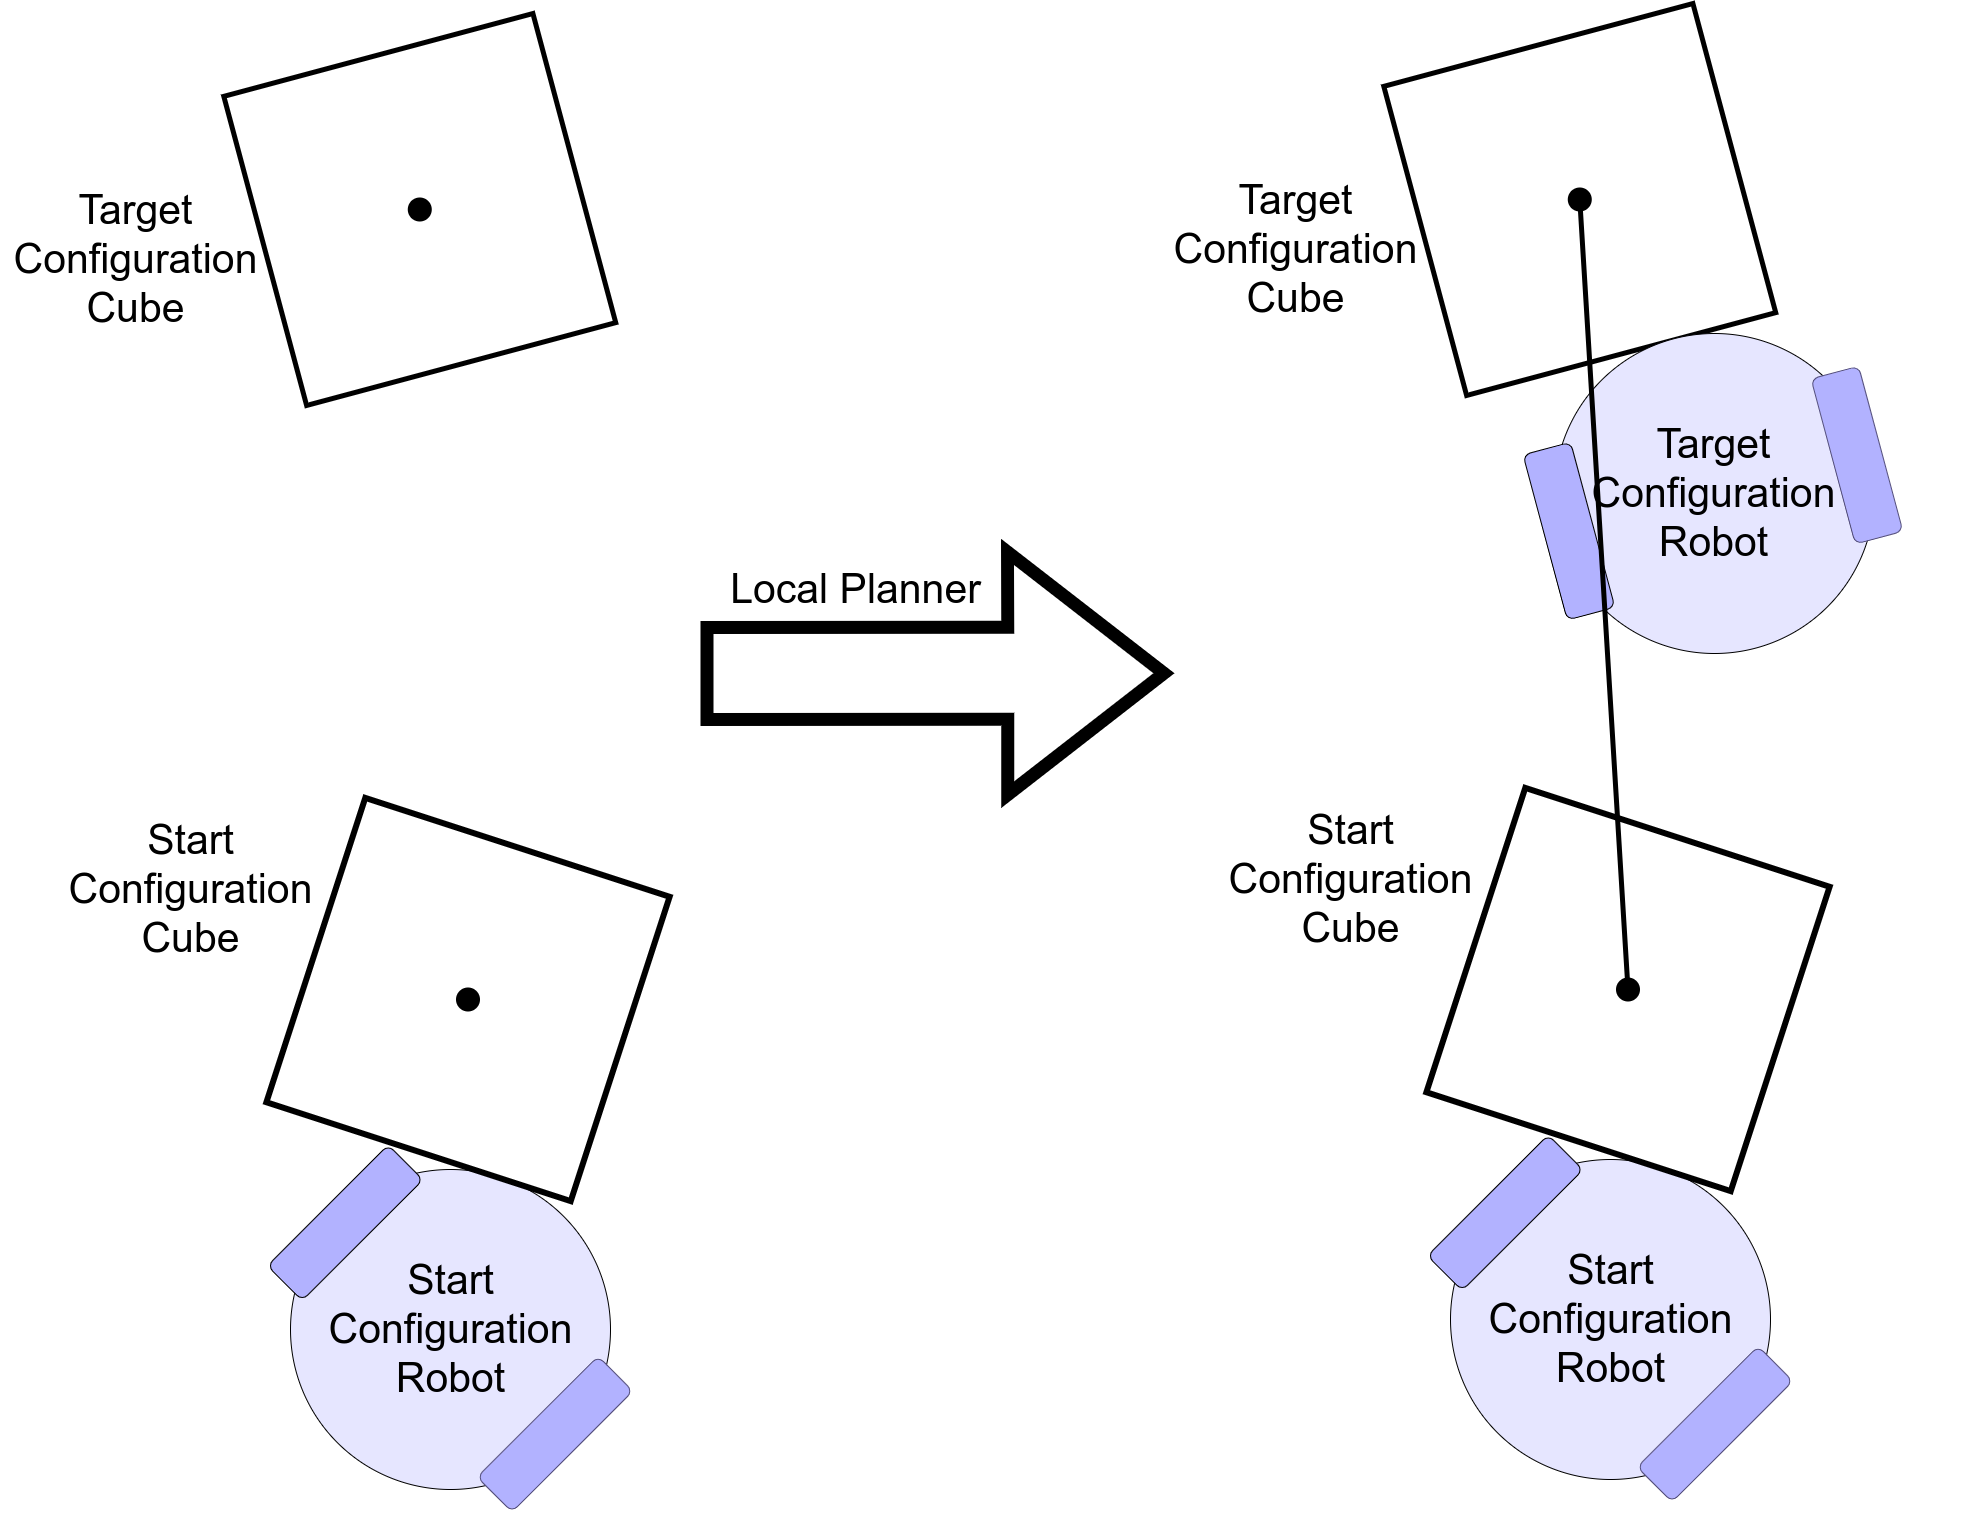
\includegraphics[width=0.6\textwidth]{figures/required_background/manipulation_local_planner}
    \caption{Generating a new robot configuration whilst adding a sample to the connectivity tree during manipulation planning.}%
    \label{fig:manipulation_plannig_local_planner}
\end{figure}

\todo{Corrado: This does not explain much. What is the strait line and how was that determines? Is that le global path ? What does the local planner arrow mean? A local planner by definition does not come up with a path to follow itself GIJS: that is about he image}
